\documentclass{beamer}

% Top-aligning columns within a top-aligned frame
% https://tex.stackexchange.com/questions/16447/beamer-top-aligning-columns-within-a-top-aligned-frame
\makeatletter
\newenvironment{myitemize}{%
   \setlength{\topsep}{0pt}
   \setlength{\partopsep}{0pt}
   \renewcommand*{\@listi}{\leftmargin\leftmargini \parsep\z@ \topsep\z@ \itemsep\z@}
   \let\@listI\@listi
   \itemize
}{\enditemize}
\makeatother  

\usepackage[USenglish]{babel}
\usepackage[utf8]{inputenc}
\usepackage{amssymb, amsmath}
\usepackage{bm}
\usepackage{color}
\usepackage{tikz}
\usepackage{url}

\definecolor{links}{HTML}{2A1B81}
\hypersetup{colorlinks,linkcolor=,urlcolor=links}

\usetheme{Boadilla}
\setbeamertemplate{headline}{}
\newcommand*\oldmacro{}%
\let\oldmacro\insertshorttitle%
\renewcommand*\insertshorttitle{%
  \oldmacro\hfill%
  \insertframenumber\,/\,\inserttotalframenumber}
  

\bibliographystyle{apalike}
% make bibliography entries smaller
%\renewcommand\bibfont{\scriptsize}
% Now get rid of all the colours
\setbeamercolor*{bibliography entry title}{fg=black}
\setbeamercolor*{bibliography entry author}{fg=black}
\setbeamercolor*{bibliography entry location}{fg=black}
\setbeamercolor*{bibliography entry note}{fg=black}

\newcommand{\lnorm}[1]{\left\lVert#1\right\rVert^2}
\newcommand{\norm}[1]{\left\lVert#1\right\rVert}

% and kill the abominable icon
\setbeamertemplate{bibliography item}{}

\begin{document}
\title{An Empirical Evaluation of Generic Convolutional and Recurrent Networks for Sequence Modeling}  
\author{Radek Bartyzal}
\date{5. 3. 2019} 
\institute{Let's talk ML in Prague}

\frame{\titlepage} 

\begin{frame}{Sequence Modeling}

Sequence Modeling:
\begin{itemize}
\item  sequence to sequence of same length
\item predict after each time step: $x_t \rightarrow y_t$
\item predictions based only on the previous elements in the sequence
\end{itemize}

\vfill

$\implies$ Not suitable for e.g. translation where 
\begin{itemize}
\item output sequence has different length
\item each element of output sequence depends on the whole input sequence = we compress the whole input sequence and then reconstruct it 
\end{itemize}


\end{frame}

%--------- END Frame 12 -------------
\begin{frame}{Dilated Causal Convolution}
\begin{figure}[h]
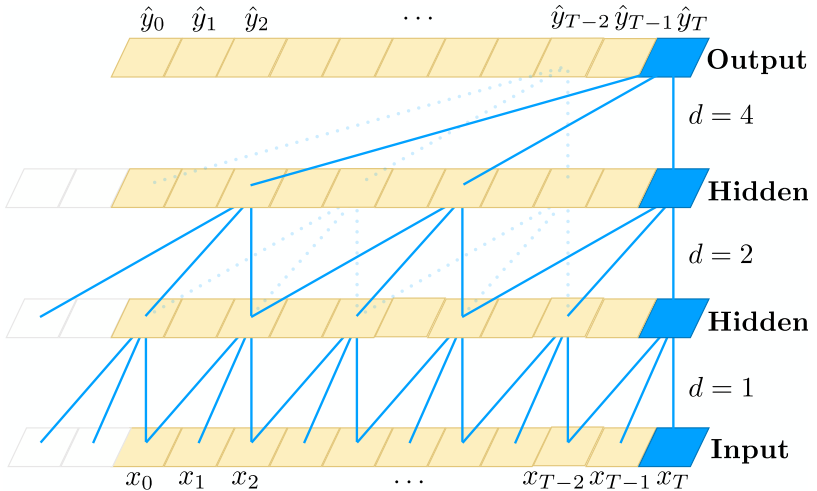
\includegraphics[width=0.8\textwidth]{img/dilated}
\caption{Dilated causal convolution with $k=3$, $d=[1, 2, 3]$. The receptive field is able to cover all values from the input sequence.}
\end{figure}
\end{frame}
%--------- END Frame 12 -------------
\begin{frame}{TCN Residual Block}
\begin{figure}[h]
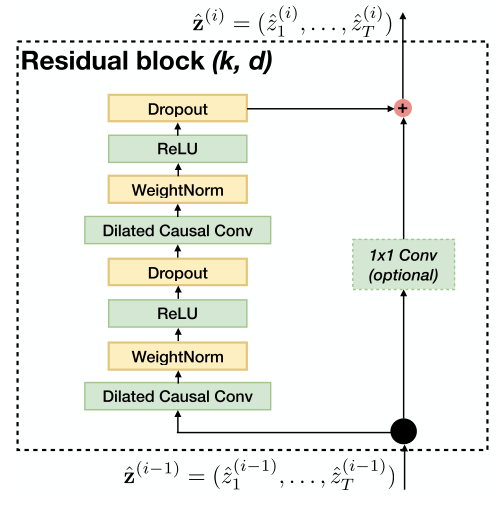
\includegraphics[width=0.55\textwidth]{img/block}
\caption{TCN residual block. An 1x1 convolution is added when residual input and output have different dimensions.}
\end{figure}
\end{frame}
%--------- END Frame 12 -------------
\begin{frame}{Generic networks results}
\begin{figure}[h]
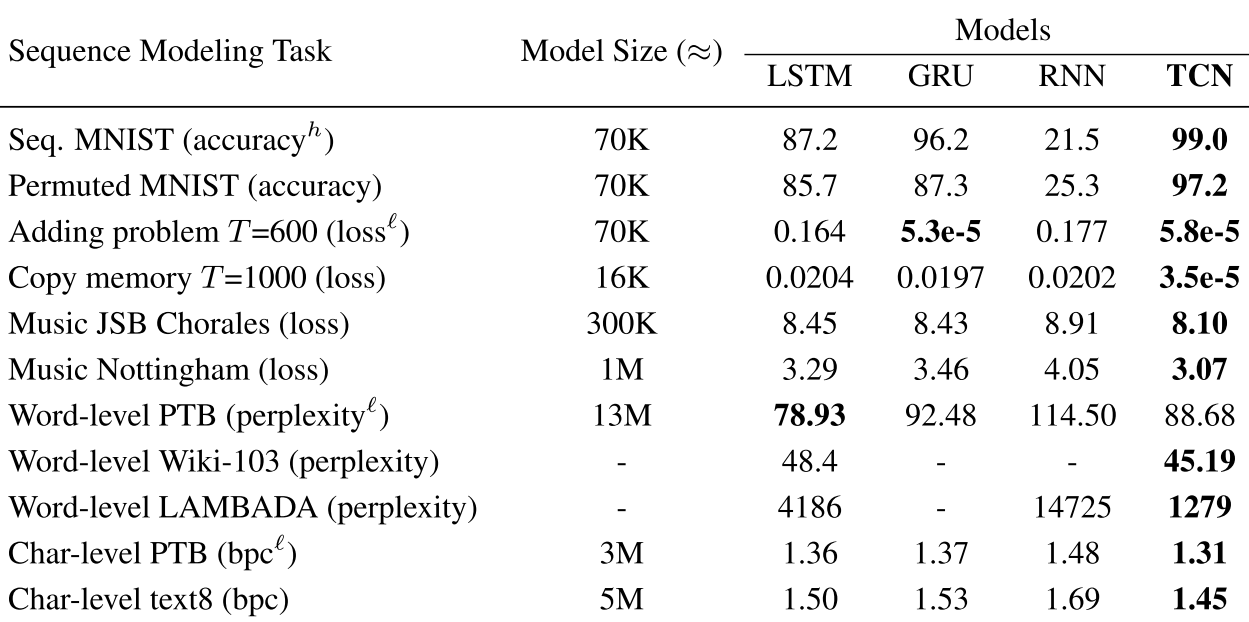
\includegraphics[width=1.0\textwidth]{img/results}
\caption{The generic TCN architecture outperforms canonical recurrent networks across a
comprehensive suite of tasks and datasets.}
\end{figure}
\end{frame}
%--------- END Frame 12 -------------
\begin{frame}{State of the art results}
\begin{figure}[h]
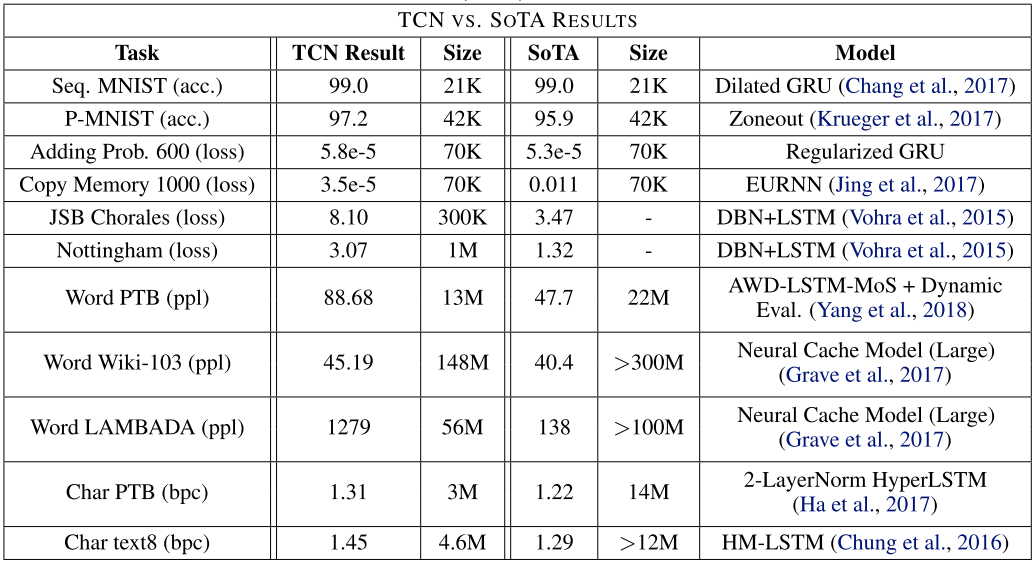
\includegraphics[width=1.0\textwidth]{img/sota}
\caption{State of the art (SOTA) results. }
\end{figure}
\end{frame}


%--------- END Frame 12 -------------
\begin{frame}{Sources}

\begin{thebibliography}{0}

  \bibitem[1]{cit:tcn} 1. Bai, Shaojie, J. Zico Kolter, and Vladlen Koltun. "An empirical evaluation of generic convolutional and recurrent networks for sequence modeling." arXiv preprint arXiv:1803.01271 (2018). \url{https://arxiv.org/abs/1803.01271} 
  
  Code: \url{https://github.com/locuslab/TCN}
  
\end{thebibliography}

\end{frame}

 
 
 
\end{document}
